\documentclass[a4paper,12pt]{book}

%Pacchetti utili
%************
%* packages *
%************

%Codifica
\usepackage[utf8]{inputenc}

%Lingua, sostituire italian con english nel caso in cui la tesi sia scritta in inglese
\usepackage[italian]{babel}

%Pacchetto per definire layout di pagina
\usepackage{fancyhdr}
\usepackage{sectsty}
\usepackage[left=3cm, right=3cm, bottom=3cm]{geometry}

%Spazia linee all'interno del documento
\usepackage{setspace}

%Listati di codice
\usepackage{verbatim}
\usepackage{listings}

%Didascalie immagini
\usepackage[hang,small,sf,font=scriptsize, labelfont=bf]{caption}
\usepackage{subcaption}

%Inclusione immagini
\usepackage{graphicx}

%Impostazioni note a piè pagina
\usepackage[stable]{footmisc}

%Citazioni e riferimenti a label
\usepackage{cite}
\usepackage[english]{varioref}

%Colori
\usepackage[usenames]{color}
\usepackage{xcolor}
\usepackage{colortbl}

%Crea link ipertestuali
\usepackage[hidelinks]{hyperref}

%Formattazione url
\usepackage{url}

%Inserimento formule
\usepackage{amsmath}
\usepackage{mathrsfs}

%Inserimento pseudocodice
\usepackage{algorithm}
\usepackage{algpseudocode}

%Citazione frasi
\usepackage{csquotes}

%Inserimento di Lorem ipsum nel testo
\usepackage{lipsum}

%\usepackage{lmodern}
\usepackage{pifont}


%Nuovi comandi
%*****************
%* nuovi comandi *
%*****************

\newcommand{\abs}[1]{\left|#1\right|}                               % modulo
\newcommand{\dato}{\left|\right.}                                   % probabilit\`{a} condizionata
\newcommand{\fun}[1]{\mathrm{#1}}                                   % stile funzione
\newcommand{\imp}{\;\;\Longrightarrow\;\;}                          % implicazione
\newcommand{\norma}[1]{\left\| #1 \right\|}                         % norma
\newcommand{\prob}[1]{\mathrm{P}\!\left[#1\right]}                  % probabilit\`{a}
\newcommand{\expect}[1]{\mathrm{E}\!\left[#1\right]}                % aspettazione
\newcommand{\sse}{\;\;\Longleftrightarrow\;\;}                      % se e solo se
\newcommand{\vect}[1]{{\boldsymbol{\mathrm{#1}}}}                   % stile vettore
\newcommand{\real}[1]{\fun{Re}\left[#1\right]}                      % parte reale
\newcommand{\imag}[1]{\fun{Im}\left[#1\right]}                      % parte immaginaria
\newcommand{\Dim}[1]{\fun{dim}\left[#1\right]}                      % dimensione di una matrice
\newcommand{\Det}[1]{\fun{det}\left[#1\right]}                      % determinante di una matrice
\newcommand{\Ker}[1]{\fun{ker}\left[#1\right]}                      % ker di una matrice
\newcommand{\rango}[1]{\fun{rango}\left[#1\right]}                  % rango di una matrice
\newcommand{\scalare}[2]{\left\langle #1, #2 \right\rangle}         % prodotto scalare
\newcommand{\blbrace}{\left  \lbrace}                               % parentesi graffa sinistra grande
\newcommand{\brbrace}{\right \rbrace}                               % parentesi graffa destra grande
\newcommand{\sinc}{\fun{sinc}}                                      % sinc
\newcommand{\rect}{\fun{rect}}                                      % rect
\newcommand{\rcos}{\fun{rcos}}                                      % rcos
\newcommand{\sgn}{\fun{sgn}}                                        % sgn
\newcommand{\N}{\mathbb{N}}                                         % insieme dei numeri naturali
\newcommand{\Z}{\mathbb{Z}}                                         % insieme dei numeri interi
\newcommand{\Q}{\mathbb{Q}}                                         % insieme dei numeri razionali
\newcommand{\R}{\mathbb{R}}                                         % insieme dei numeri reali
\newcommand{\C}{\mathbb{C}}                                         % insieme dei numeri complessi
\newcommand{\seq}[2][n]{#2_{0}, #2_{1}, \ldots, \, #2_{#1}}         % sequenza
\newcommand{\Span}[2][n]
{\fun{span} \blbrace #2_{1}, #2_{2}, \ldots, \, #2_{#1} \brbrace}   % spazio generato
\newcommand{\ddt}{\frac{\fun{d}}{\fun{dt}}}                         % derivata
\newcommand{\Div}[2]{#1 \; \mid \; #2}                              % divide
\newcommand{\MCD}[2]{\fun{MCD}\(#1, #2\)}                           % massimo comun divisore
\newcommand{\mcm}[2]{\fun{mcm}\(#1, #2\)}                           % minimo comune multiplo
\newcommand{\goodgap}{
                      \hspace{\subfigtopskip}
                      \hspace{\subfigbottomskip}
                     }                                              % interlinea opportuna per le sottofigure
\newcommand{\eng}[1]{\emph{#1}}                                   % inglese
\newcommand{\virg}[1]{``#1"}                                        % fa una citazione tra virgolette
%\newcommand{\unit}[2]($\frac{\text{#1}}{\text{#2}}$)                % unit\`{a} di misura
\newcommand{\textttvar}[1]{{\ttvar #1}}

\definecolor{gray}{gray}{0.9}
\newcommand{\listato}[1]{\lstset{language=#1, numbers=left, numberstyle=\tiny, stepnumber=2, numbersep=5pt, numberblanklines=false, xleftmargin=5pt, captionpos=b, stringstyle=\ttfamily, columns=flexible, showstringspaces=false, tabsize=2, frame=single, framerule=0pt, backgroundcolor=\color{gray}, basicstyle=\small}}

%****************************
%* ridefinizioni di comandi *
%****************************

\renewcommand{\(}{\left(}                                     % parentesi tonda sinistra grande
\renewcommand{\)}{\right)}                                    % parentesi tonda destra grande
\renewcommand{\[}{\left[}                                     % parentesi quadra sinistra grande
\renewcommand{\]}{\right]}                                    % parentesi quadra destra grande
\renewcommand{\exp}[1]{\fun{e}^{#1}}                          % esponenziale
\renewcommand{\gcd}[2]{\fun{gcd}\(#1, #2\)}                   % massimo comun divisore

\renewcommand{\lstlistingname}{Listing}
\renewcommand{\lstlistlistingname}{Elenco dei listati codice}

\makeatletter
\def\BState{\State\hskip-\ALG@thistlm}
\makeatother

%Definizione input e output pseudocodice
\renewcommand{\algorithmicrequire}{\textbf{Input:}}
\renewcommand{\algorithmicensure}{\textbf{Output:}}
 
%"Nome" della bibliografia
\addto{\captionsenglish}{%
  \renewcommand{\bibname}{References}
}

%Impostazioni dei margini, definizione di colori e di stili vari
\newfont{\ttvar}{cmvtt10 scaled 1200}     % nuovo carattere tipi courier a spaziatura variabile per le dimostrazioni

% margini senato
\textwidth       =  14.50 cm            % larghezza 21 cm - 4 cm (sinistro) - 2.5 (destro)
\textheight      =  23.10 cm            % altezza 29.7 cm - 3 cm (superiore) - 2 (inferiore)
\topmargin       =   0.00 cm            % margine superiore 3 cm diminuito di 1 inch
\oddsidemargin   =   1.46 cm            % margine sinistro 4 cm diminuito di 1 inch
\evensidemargin  =  -0.04 cm            % margine destro 2.5 cm diminuito di un inch

\setlength{\headsep}{1.0cm}
\setlength{\footskip}{1.0cm}
\parindent = 0.7cm
\captionmargin = 0.7cm

%Interlinea 1.5
\onehalfspacing

% stile pagina
\pagestyle{fancy}
\renewcommand{\chaptermark}[1]{\markboth{\chaptername\ \thechapter.\ #1 }{}}
\renewcommand{\sectionmark}[1]{\markright{\thesection\ #1}{}}
\fancyhead{}
\fancyhead[LE,RO]{\sffamily \thepage}
\fancyhead[RE]{\sffamily \leftmark}
\fancyhead[LO]{\sffamily \rightmark}
\fancyfoot{}

% ridefinisco lo stile plain
\fancypagestyle{plain}{ \fancyhead{} \fancyfoot{}
\fancyfoot[C]{\sffamily \thepage}
\renewcommand{\headrulewidth}{0pt}}

% stile per i titoli
\allsectionsfont{\sffamily \raggedright}

% definisco i colori
\definecolor{codegreen}{rgb}{0,0.6,0}
\definecolor{codegray}{rgb}{0.5,0.5,0.5}
\definecolor{codepurple}{rgb}{0.58,0,0.82}
\definecolor{backcolour}{rgb}{0.95,0.95,0.92}
\definecolor{backcolourwhite}{rgb}{1,1,1}

%definisco stile listati di codice
\lstdefinestyle{mystyle}{
    %backgroundcolor=\color{backcolour},   
    commentstyle=\color{codegreen},
    keywordstyle=\color{magenta},
    numberstyle=\tiny\color{codegray},
    stringstyle=\color{codepurple},
    basicstyle=\ttfamily\footnotesize,
    breakatwhitespace=false,         
    breaklines=true,                 
    captionpos=b,                    
    keepspaces=true,                 
    numbers=left,                    
    numbersep=5pt,                  
    showspaces=false,                
    showstringspaces=false,
    showtabs=false,                  
    tabsize=2,
    xleftmargin=.07\textwidth, %xrightmargin=.2\textwidth
}

\lstset{style=mystyle}
\lstset{emph={RandomForestClassifier, RandomizedSearchCV, GridSearchCV},emphstyle=\underbar}



\begin{document}
\begin{titlepage}
\begin{center}
%
\includegraphics[scale=0.1]{images/logo.png}\\

%Per il frontespizio del dipartimenti di Ing. dell'Informazione commentare le riga precedente e decommentare la successiva

\includegraphics[scale=0.2]{images/logo_unipd.png} \hfill 
\includegraphics[scale=0.2]{images/logo_dei.png}\\
\vspace{0.8cm}
\textsc{\LARGE Universit\`{a} degli Studi di Padova}\\
\vspace{0.45cm}
\textsc{\large Dipartimento di Ingegneria dell'Informazione}\\
\vspace{0.4cm}
\textsc{\large Corso di Laurea Triennale in}\\
\textsc{\large Ingegneria Informatica}\\
\vfill
% Title
{ \LARGE \bfseries Analisi dei sensori coppia-forza per lo sviluppo di applicazioni industriali in ROS
}\\
\vfill
\textit{\large Relatore:} \hfill \textit{\large Laureando:}\\
\textsc{\large Prof. Stefano Ghidoni} \hfill \textsc{Andrea Stocco}\\
\textit{\large Correlatore:} \hfill \textsc{2009353}\\
\textsc{\large Matteo Terreran, PhD} \hfill \textit{}

\vfill
% Bottom of the page
{\large Anno Accademico 2022/2023}
\end{center}
\end{titlepage}

\thispagestyle{empty} %pagina bianca dopo il titolo
\cleardoublepage

\pagenumbering{Roman} %numerazione romana per l'indice, l'abstract e i ringraziamenti
\thispagestyle{empty}

\clearpage{\pagestyle{plain}\cleardoublepage}
%definisco il layout dell'abstract
\def\changemargin#1#2{\list{}{\rightmargin#2\leftmargin#1}\item[]}
\let\endchangemargin=\endlist

%Genero l'ambiente per l'abstract
\newcommand\summaryname{Abstract}
\newenvironment{Abstract}%
    {\begin{center}%
    \bfseries{\summaryname} \end{center}}

\begin{Abstract}
%\begin{changemargin}{1cm}{1cm}
    I sensori coppia-forza sono componenti fondamentali nei sistemi robotici in quanto forniscono dati sulle forze e i momenti 
    esterni applicati al robot. Questi dati possono essere utilizzati per applicazioni a supporto della collaborazione uomo-robot 
    e per l'automatizzazione di attivit\'{a} che richiedono elevata precisione. ROS (Robot Operating System) \'{e} un framework che 
    fornisce una vasta gamma di librerie e strumenti software per lo sviluppo di applicazioni robotiche. In questa tesi verranno 
    mostrate delle possibili applicazioni ROS in ambito industriale per i sensori coppia-forza, dopo averli validati attraverso 
    alcuni esperimenti.
%\end{changemargin}
\end{Abstract}

\clearpage{\pagestyle{plain}\cleardoublepage}
\tableofcontents %Indice

\clearpage{\pagestyle{plain}\cleardoublepage} %Numerazione araba per i capitoli
\pagenumbering{arabic}

\clearpage{\pagestyle{plain}\cleardoublepage} %Comando per iniziare il capitolo su pagina dispari
\chapter*{Introduzione} %Nome capitolo
\addcontentsline{toc}{chapter}{Introduzione} 
I robot manipolatori hanno rivoluzionato l'automazione industriale, permettendo lo svolgimento
di operazioni complesse in modo rapido, preciso e sicuro. 
Uno dei modelli pi\'{u} utilizzato \'{e} l'\textbf{UR5} di \textbf{Universal Robot}. Per via della sua flessibilit\'{a} 
ed efficienza si \'{e} scelto di utilizzarlo in questo studio. 
Un ruolo chiave nel controllo di questi robot viene assunto dai sensori coppia-forza,
che permettono di misurare e regolare la forza esercitata dal robot durante lo svolgimento delle proprie attivit\'{a}. 
La loro versatilit\'{a} li rende strumenti preziosi in molti campi tra cui: la \textbf{robotica industriale} e la \textbf{medicina}. 
Essi infatti consentono al robot di controllare la forza esercitata durante le operazioni di assemblaggio, levigatura, 
saldatura e manipolazione degli oggetti. Vengono inoltre utilizzati nella riabilitazione, per valutare la forza muscolare 
e i progressi del paziente.
% aggiungere foto levigatura e riabilitazione
Questi sensori sono in grado di convertire le forze e le coppie applicati ad essi in segnali elettrici che possono essere 
interpretati da altri dispositivi. 
Esistono varie tipologie di sensori coppia-forza, ognuna delle quali ha un diverso meccanismo di funzionamento. 
I sensori \textbf{piezoelettrici} sfruttano la propriet\'{a} di alcuni materiali (cristalli piezoelettrici) 
di generare una carica elettrica se sottoposti a deformazione meccanica. Tale variazione  
pu\'{o} essere misurata per determinare la forza o la coppia applicata.
Il sensore \textbf{FT 300-S} di \textbf{Robotiq} sfrutta questo principio di funzionamento ed \'{e} in grado di misurare 
forze e coppie lungo i sei gradi di libert\'{a} (x, y, z, roll, pitch, yaw). 
\'{E} stato necessario installarlo manualmente sull'UR5 perch\'{e}, a differenza di altri, non possiede sensori 
coppia-forza integrati. 
In questa tesi verr\'{a} presentata l'implementazione di un sistema di controllo della forza per l'UR5 utilizzando i dati
forniti dall'FT 300-S e il framework di sviluppo \textbf{ROS (Robot Operating System)}.
ROS \'{e} ampiamente utilizzato dalla comunit\'{a} informatica perch\'{e} fornisce strumenti e librerie 
per il controllo e la comunicazione tra le componenti di un sistema robotico.
Alcuni test per la valutazione delle prestazioni del sensore in termini di reattivit\'{a} e precisione verranno descritti nel Capitolo 
\ref{chapter:chapter4}.
Nel Capitolo \ref{chapter:chapter5}, invece, verranno presentate delle possibili applicazioni volte a dimostrare l'efficacia
di tali sensori per lo svolgimento di attivit\'{a} industriali, come il \textbf{pick and place} e il \textbf{trasporto collaborativo}.
 %File in cui verrà scritto il capitolo

\clearpage{\pagestyle{plain}\cleardoublepage} %Comando per iniziare il capitolo su pagina dispari
\chapter{ROS} %Nome capitolo
\label{chapter:chapter1} %Label per creare riferimenti al capitolo
ROS (Robot Operating System) \'{e} un framework open-source di Python e C++ per lo sviluppo di applicazioni robotiche.
Ne esistono varie versioni, quella raccomandata e utilizzata in questa tesi \'{e} ROS Noetic per Ubuntu Focal 20.04.
Questo capitolo ci fornir\'{a} una panoramica esaustiva del Robot Operating System e dell'ambiente di esecuzione associato 
\cite{ros}.

\section{Workspace}
Per poter eseguire codice ROS abbiamo bisogno di un ambiente che permetta l'organizzazione e l'utilizzo di tutti i nostri pacchetti.
Catkin \'{e} il sistema di compilazione ufficiale di ROS che ci consente di creare un workspace per organizzare 
e gestire le nostre applicazioni.
I termini `pacchetto' e `applicazione' sono interscambiabili e possono essere utilizzati in modo equivalente (una definizione pi\'{u} 
rigorosa verr\'{a} data nel corso di questo capitolo).
Una volta creato il workspace catkin \cite{catkin_ws}, saremo in grado di compilare il codice sorgente contenuto all'interno 
dei nostri pacchetti.


\section{Nodo}
Un \textbf{nodo} \'{e} un eseguibile che sfrutta ROS per comunicare con altri nodi.
Quando viene lanciato il comando \verb|catkin_make|, ogni file sorgente in ogni pacchetto viene compilato 
dando origine ad un nodo.
Impropriamente, si potrebbe quindi dire che un pacchetto \'{e} un insieme di nodi riguardanti la stessa applicazione.
Per poter eseguire un nodo \'{e} sufficiente eseguire il comando \\
\verb|rosrun <nome_pacchetto> <nome_nodo>|. 
Prima di eseguirne uno \'{e} necessario, tuttavia, avviare un ROS Master.
Lo scopo principale di un \textbf{ROS Master} \'{e} quello di consentire ai singoli nodi di localizzarsi a vicenda. Una volta 
fatto partire, essi potranno comunicare tra loro attraverso topic o service.
Per eseguire un ROS Master sar\'{a} sufficiente eseguire il comando \verb|roscore| in un altro terminale.


\section{Topic}
I topic sono dei canali di comunicazione unidirezionali che consentono lo scambio di informazioni tra nodi sottoforma di 
messaggi. Un nodo che pubblica messaggi su un topic viene chiamato publisher, mentre un nodo che legge i messaggi da un topic 
viene chiamato subscriber.
\begin{figure}[H]
    \centering
    \includegraphics*[width=0.75\textwidth]{images/topic_graph.png}
    \caption{Schema di comunicazione}
    \label{fig:topic_graph}
\end{figure}
Per pubblicare un messaggio su un topic bisogna utilizzare l'apposita funzione \verb|publish()| passandole come parametro 
il messaggio che vogliamo pubblicare.
A discapito del nome, questa funzione non pubblica effettivamente il messaggio, ma lo mette in una coda d'attesa (la cui 
dimensione viene specificata quando viene istanziato il publisher).
Un thread separato si occupa di inviare effettivamente il messaggio al topic per renderlo visibile a tutti i nodi subscriber 
connessi.
Se il numero di messaggi in coda supera la dimensione di essa, i messaggi pi\'{u} vecchi verranno cancellati per fare spazio 
a quelli pi\'{u} recenti. Quando arriva un nuovo messaggio al subscriber, esso viene salvato 
in una coda d'attesa (stesso funzionamento di quella del publisher) fino a quando ROS non d\'{a} la possibilit\'{a} al nodo 
di eseguire la funzione di callback. Tale funzione \'{e} definita dall'utente e si occupa di processare il messaggio ricevuto. 
ROS eseguir\'{a} una callback solo quando gli daremo il permesso di farlo. Ci sono due modi per fare ci\'{o}:
\begin{itemize}
    \item \verb|ros::spinOnce()| chiede a ROS di eseguire tutte le callback in sospeso e poi ci restituisce il controllo
    \item \verb|ros::spin()| chiede a ROS di attendere e di eseguire tutte le callback in sospeso fino a quando il nodo non 
          viene spento. \'{E} equivalente a:
          \begin{verbatim}
            while (ros::ok()) {
                ros::spinOnce();
            }
          \end{verbatim} 
          \verb|ros::ok()| ritorna 0 quando: 
          \begin{itemize}
            \item il nodo viene spento attraverso un SIGINT (Ctrl-C) oppure dalla chiamata di \verb|ros::shutdown()| in 
                  un altro punto del codice
            \item un altro nodo con lo stesso nome viene eseguito
          \end{itemize}
\end{itemize}
In altre parole \verb|ros::spin()| vincola il nodo a rimanere sempre e solo in attesa di leggere nuovi messaggi. 
Se il nodo non deve solamente eseguire le callback, allora un loop con \verb|ros::spinOnce()| \'{e} la scelta corretta.
(Aggiungere link ad un mio pacchetto di esempio???)
 %File in cui verrà scritto il capitolo

\clearpage{\pagestyle{plain}\cleardoublepage} %Comando per iniziare il capitolo su pagina dispari
\chapter{Ambiente di lavoro} %Nome capitolo
\label{chapter:chapter2} %Label per creare riferimenti al capitolo
Il sensore FT300-S di Robotiq \'{e} stato installato all'estremit\'{a} dell'UR5 e collegato alla control box per ricevere 
l'alimentazione necessaria. 
\begin{figure}[H]
    \centering
    \includegraphics*[width=0.5\textwidth]{images/ft.png}
    \caption{FT300-S}
    \label{fig:ft}
\end{figure}
\'{E} importante notare come la sua presenza non precluda la possibilit\'{a} di installazione di un end effector, 
che pu\'{o} essere facilmente posizionato `al di sopra' del sensore. 
L'FT300-S \'{e} in grado di rilevare forze e torsioni nel range di $\pm 300 N$ e $\pm 30 Nm$ rispettivamente. 
Le misurazioni del sensore hanno un rumore di fondo intrinseco, \'{e} quindi necessario scartare tutti i dati al di sotto delle 
soglie consigliate nel manuale \cite{ft_sensor} in quanto non attendibili. 
Per collegare il sensore al PC sono state provate due alternative: 
\begin{itemize}
    \item collegamento via USB tra sensore e control box e via ethernet tra control box e computer
    \item collegamento diretto via USB tra sensore e computer
\end{itemize}

\subsection{Collegamento via USB tra sensore e control box e via ethernet tra control box e computer}
\begin{figure}[H]
    \centering
    \includegraphics*[width=0.1\textwidth]{images/ft-cbox-pc.png}
    \caption{Schema collegamento}
    \label{fig:ft-cbox-pc}
\end{figure}
bla bla bla

\subsection{Collegamento diretto via USB tra sensore e computer}
\begin{figure}[H]
    \centering
    \includegraphics*[width=0.1\textwidth]{images/ft-pc.png}
    \caption{Schema collegamento}
    \label{fig:ft-pc}
\end{figure}
bla bla bla

 %File in cui verrà scritto il capitolo

\clearpage{\pagestyle{plain}\cleardoublepage} %Comando per iniziare il capitolo su pagina dispari
\chapter{Validazione del sensore} %Nome capitolo
\label{chapter:chapter3} %Label per creare riferimenti al capitolo
In questo capitolo verranno mostrati degli esperimenti per valutare il funzionamento e le prestazioni del sensore. 
Per l'analisi della \textbf{reattivit\'{a}}, viene osservato il comportamento del sensore nel caso in cui ci sia 
un cambiamento istantaneo delle forze in gioco. 
Un'altro importante aspetto da valutare \'{e} la \textbf{precisione} dei dati forniti dal sensore. Per farlo 
si \'{e} pensato di utilizzare le misurazioni effettuate per calcolare la viscosit\'{a} di un liquido di cui se ne conosce 
il valore. 
Prima di mostrare i risultati di questi due esperimenti \'{e} bene, per\'{o}, parlare dell'importanza dell'azzeramento periodico 
del sensore.

\section{Errore nelle misurazioni}
Come spiegato nel Capitolo \ref{chapter:chapter2}, il sensore \`{e} soggetto a rumore di fondo intrinseco che 
pu\`{o} essere causato da diversi fattori, come la temperatura, l'instabilit\`{a} dell'alimentazione o il rumore elettrico. 
\newpage
\begin{figure}[H]
    \centering
    \includegraphics*[width=0.80\textwidth]{images/drifting.png}
    \caption{Drifting lungo l'asse z}
    \label{fig:drifting}
\end{figure}
In Figura \ref{fig:drifting} viene mostrato il fenomeno del \textbf{drifting}: ossia quando un sensore nel corso del tempo 
mostra una deviazione nelle sue letture senza un'effettiva variazione delle condizioni ambientali. Questo fenomeno si verifica 
solamente se il sensore viene collegato al PC come indicato nella Sezione \ref{sec:scp}. 
Si pu\`{o} notare come la forza rilevata dal sensore lungo l'asse z decresca per i primi 250 secondi, per poi 
cominciare una fase di crescita lineare senza che al sensore venga applicata alcuna forza. 
La forza misurata supera la soglia di confidenza specificata nel manuale entro la 
quale la misurazione deve essere catalogata come non attendibile. 
Per ovviare a questo problema, nel caso in cui si optasse per un collegamento passante per la control box del robot, 
sarebbe necessario azzerare il sensore periodicamente in modo che le letture risultino corrette e senza deviazioni. 
Gli esperimenti descritti nel corso di questo capitolo e le applicazioni presenti nel Capitolo \ref{chapter:chapter5}, sono state 
sviluppate utilizzando un collegamento diretto tra sensore e PC via USB.


\section{Taglio del filo}
Al fine di valutare la reattivit\`{a} del sensore coppia-forza, \`{e} stato condotto un esperimento per esaminare la capacit\`{a} del 
sensore di rilevare rapidamente una variazione istantanea della forza. 
Tale variazione improvvisa \`{e} stata simulata 
tagliando un filo che sosteneva un oggetto appeso al sensore. La misurazione rilevata a seguito del taglio  
deve mostrare una variazione \textbf{proporzionale al peso dell'oggetto}.
In questo esperimento, \`{e} stato attaccato al sensore un filo con appeso un oggetto di 0.155 Kg. 
Il braccio \`{e} stato posizionato in modo tale che la forza peso gravasse solo su un asse del sensore alla volta, cosicch\`{e} 
il valore rilevato dopo il taglio fosse compatibile con il peso dell'oggetto precedentemente attaccato. 
In Figura \ref{fig:setup_z}, viene mostrato il setup per l'esperimento lungo l'asse z. 
\newpage
\begin{figure}[H]
    \centering
    \begin{subfigure}[b]{0.4\textwidth}
        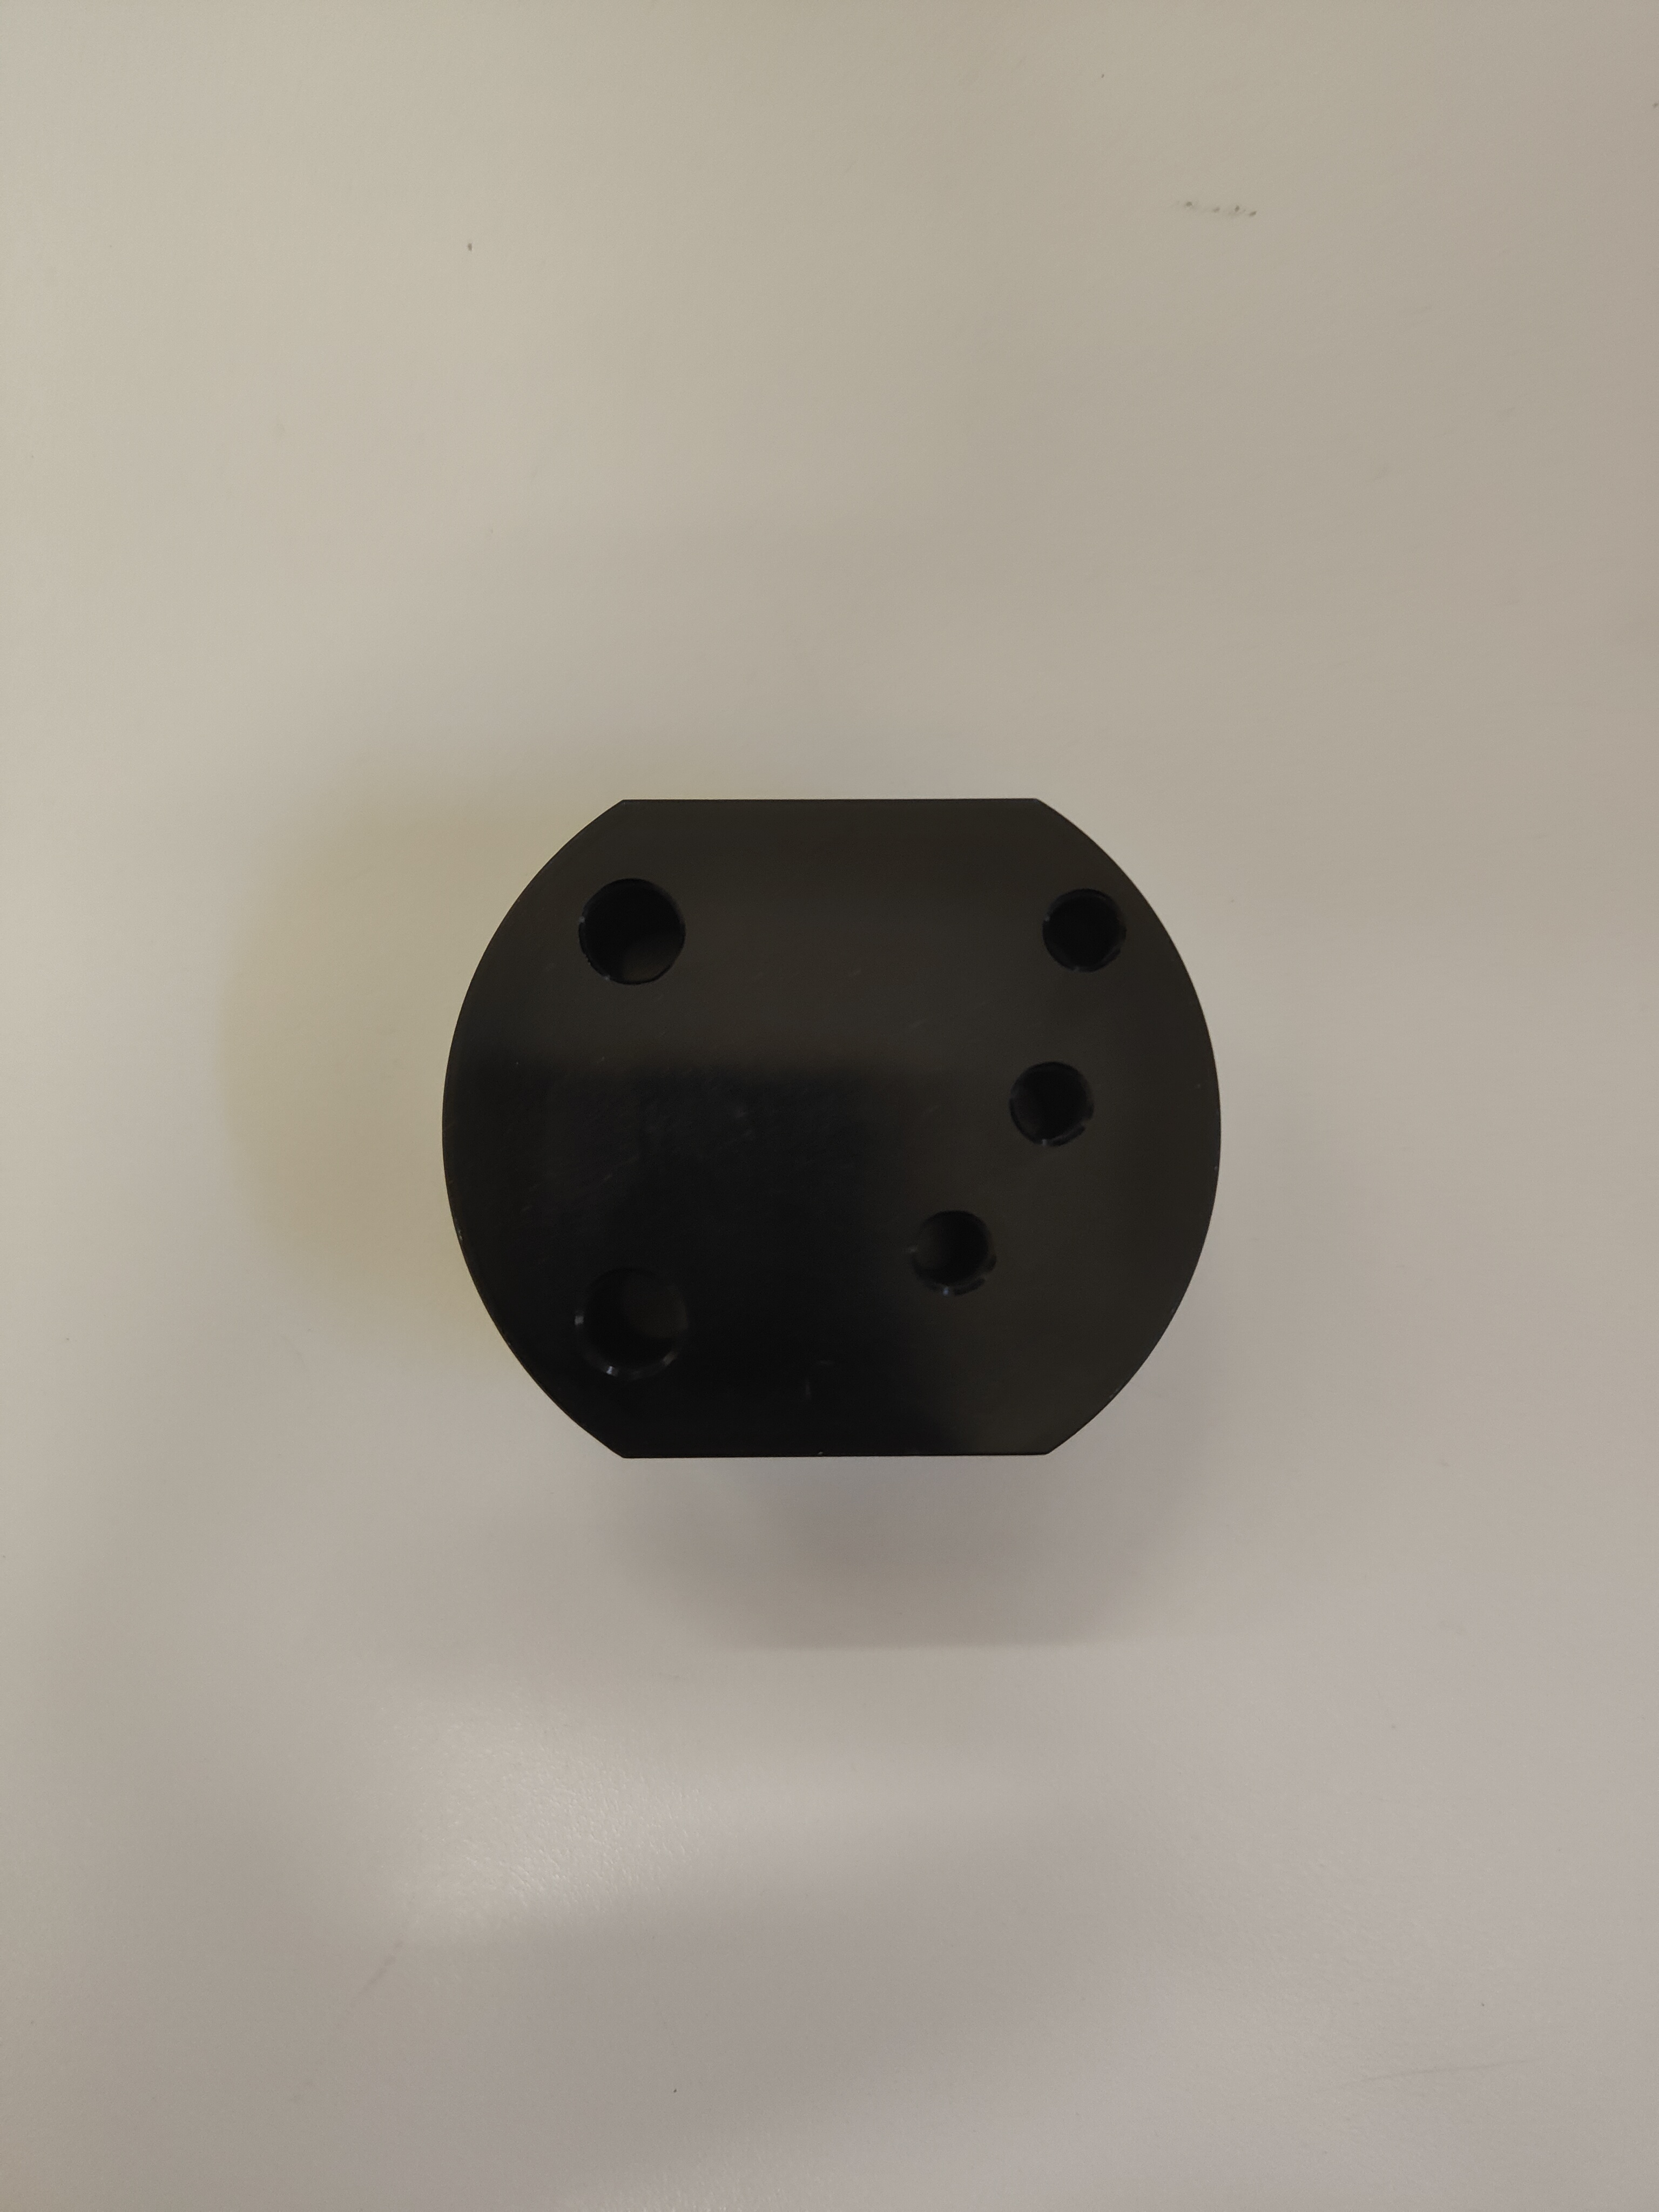
\includegraphics[width=\textwidth]{images/object.jpg}
        \label{fig:object}
    \end{subfigure}
    \qquad
    \begin{subfigure}[b]{0.4\textwidth}
        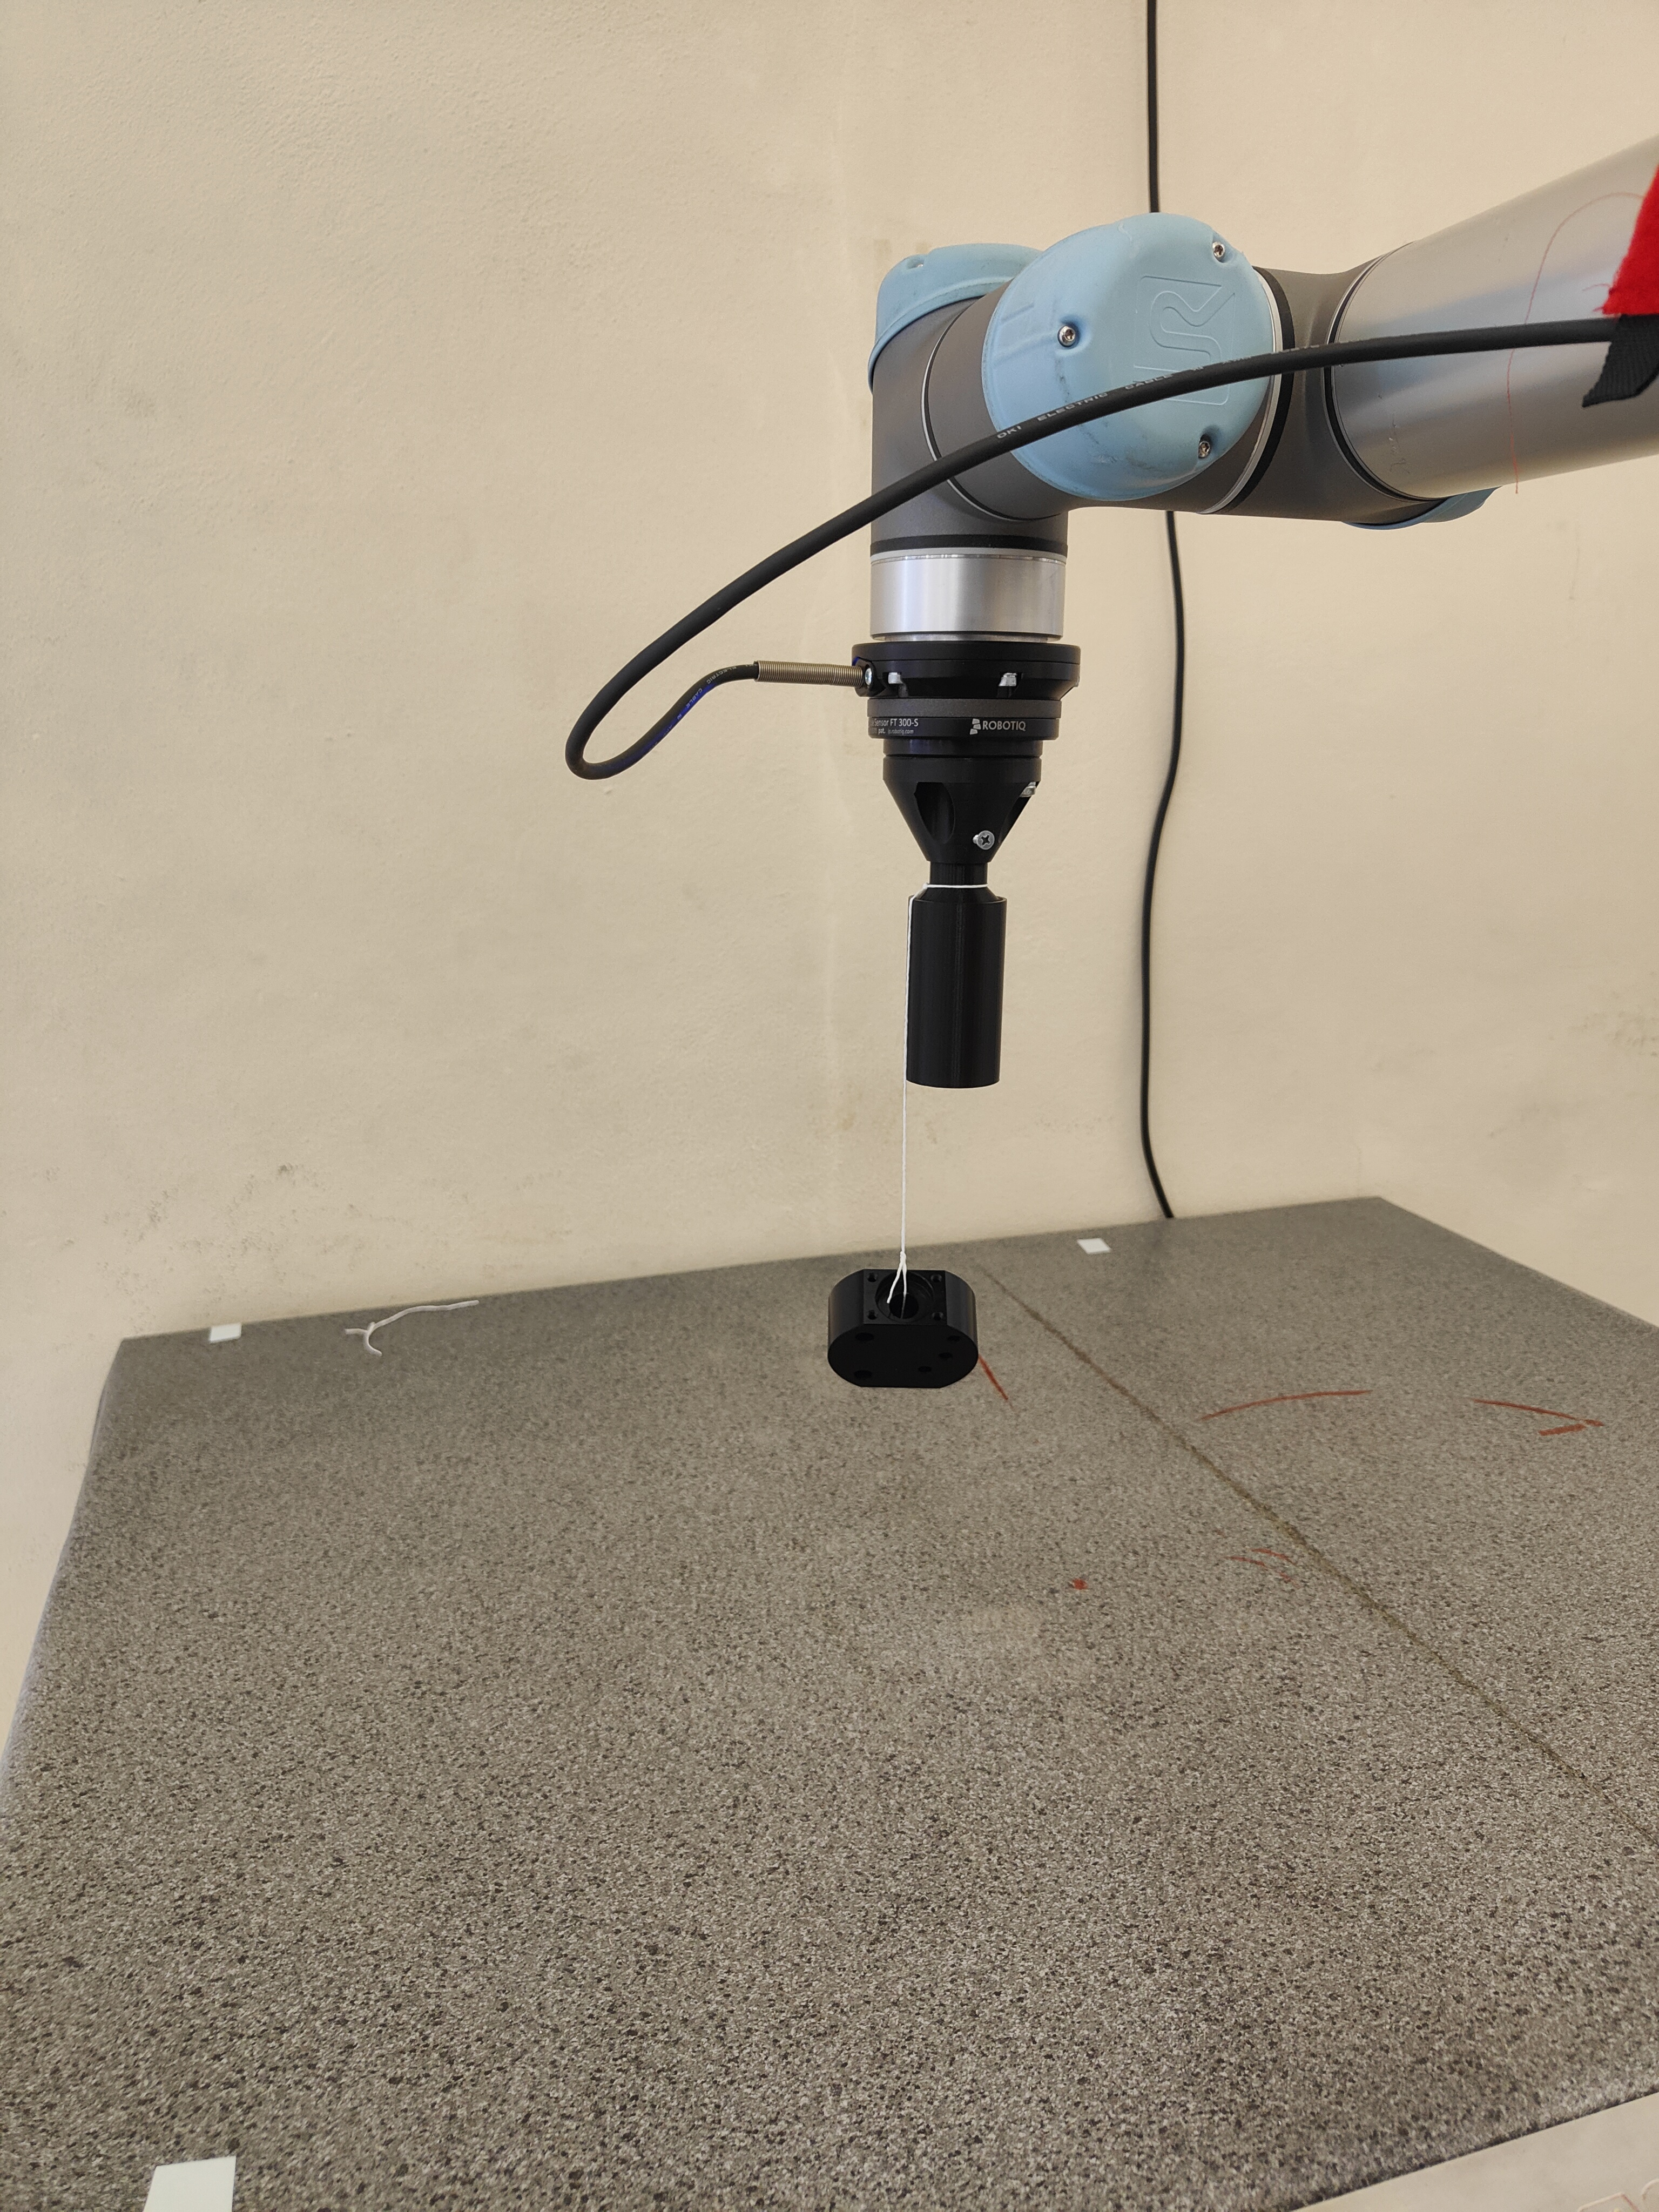
\includegraphics[width=\textwidth]{images/setup_z.jpg}
        \label{fig:setup}
    \end{subfigure}
    \caption{Setup sperimentale per l'analisi della reattivit\`{a}. A sinistra, l'oggetto di metallo utilizzato, 
    a destra l'oggetto collegato con un filo al robot (forza peso che grava sull'asse z del sensore)}\label{fig:setup_z}
\end{figure}
Dopo aver azzerato il sensore, per verificarne la reattivit\`{a}, il filo \`{e} stato tagliato di netto. 
Il taglio del filo \`{e} un ottimo modo per `simulare' un cambiamento di forza istantaneo.
\begin{figure}[H]
    \centering
    \includegraphics*[width=0.85\textwidth]{images/z_cut.png}
    \caption{Andamento taglio del filo misurato lungo l'asse z del sensore coppia-forza}
    \label{fig:z_cut}
\end{figure}
In Figura \ref{fig:z_cut} viene mostrato l'andamento della forza rilevata dal sensore lungo l'asse z. 
Si pu\`{o} notare che, fino a quando il filo \`{e} attaccato al sensore, la forza rilevata \`{e} circa zero. 
Questo perch\'{e} il sensore \`{e} stato azzerato quando l'oggetto era gi\`{a} stato appeso al sensore. 
Nel momento in cui avviene il taglio, il grafico si allinea istantaneamente al peso reale dell'oggetto, 
ossia circa 1.5 N (il valore previsto dovrebbe essere $0.155 \text{ Kg} \cdot 9.81 \frac{\text{N}}{\text{Kg}} = 1.52055 \text{ N}$).
Tale esperimento \`{e} stato ripetuto anche per gli altri due assi, confermando lo stesso valore indicativo di -1.5 N.
\begin{figure}[H]
    \centering
    \includegraphics*[width=0.45\textwidth]{images/setup_x.jpg}
    \caption{Setup sperimentale per l'analisi della reattivit\`{a} lungo l'asse x del sensore coppia-forza}
    \label{fig:setup_x}
\end{figure}
Muovendo il robot nella configurazione mostrata in Figura \ref{fig:setup_x}, la forza peso dell'oggetto grava univocamente sull'asse x 
del sensore. 
Ruotando l'end effector di 90° si ottiene il setup equivalente per l'asse y.
I risultati vengono mostrati in Figura \ref{fig:x_cut} e \ref{fig:y_cut}. 
\begin{figure}[H]
    \centering
    \includegraphics*[width=0.85\textwidth]{images/x_cut.png}
    \caption{Andamento taglio del filo misurato lungo l'asse x del sensore coppia-forza}
    \label{fig:x_cut}
\end{figure}
\begin{figure}[H]
    \centering
    \includegraphics*[width=0.85\textwidth]{images/y_cut.png}
    \caption{Andamento taglio del filo misurato lungo l'asse y del sensore coppia-forza}
    \label{fig:y_cut}
\end{figure}
A differenza di quanto riportato nei primi due grafici, l'andamento della forza rilevata lungo l'asse y, presenta un picco 
anomalo dovuto al taglio non sufficientemente netto del filo.


\section{Calcolo della viscosit\'{a}}
In questa sezione viene mostrato un esperimento per valutare la precisione delle misurazioni del sensore\footnotemark{}. 
Per farlo si \'{e} pensato di usare i momenti angolari misurati dal sensore per calcolare la \textbf{viscosit\'{a}} del burro 
d'arachidi e confrontarla con il valore ufficiale noto (150-250 $\text{Pa} \cdot \text{s}$). 
A tal proposito \'{e} stato installato sull'UR5 un cilindro (di raggio 2cm e altezza 7.5cm) come end effector. 
Si \'{e} scelto di utilizzare un tool con questa forma per agevolare la determinazione della formula dell'attrito viscoso agente 
in questo caso.
In Figura \ref{fig:peanut_butter} viene mostrato il setup per questo esperimento. 
\newpage
\begin{figure}[H]
    \centering
    \includegraphics*[width=0.45\textwidth]{images/setup_viscosity.jpg}
    \caption{Setup sperimentale per l'analisi della precisione, composto da un vasetto di burro d'arachidi e un tool 
    cilindrico stampato in 3D}
    \label{fig:peanut_butter}
\end{figure}
Il cilindro, una volta immerso nel burro di arachidi, viene fatto ruotare attorno al suo asse con velocit\'{a} angolare 
costante. Il sensore, rileva quindi un momento torcente lungo l'asse z corrispondente alla forza di attrito viscoso esercitata 
dal fluido sul cilindro in rotazione. \'{E} dunque possibile utilizzare tali valori per ricavare sperimentalmente 
la viscosit\'{a} del burro d'arachidi e confrontarla con i dati ufficiali noti. 
La formula per il calcolo dell'attrito viscoso \'{e} la seguente 
\begin{equation*}
    M = 2\pi \cdot \eta \cdot \frac{\omega \cdot h}{\Delta r} \cdot r_{1}^{3}
\end{equation*}
con 
\begin{itemize}
    \item $\eta$: viscosit\'{a} del fluido
    \item $\omega$: velocit\'{a} angolare di rotazione
    \item h: altezza del cilindro
    \item $r_{1}$: raggio del cilindro
    \item $r_{2}$: raggio del barattolo
    \item $\Delta r$: $r_{2} - r_{1}$
\end{itemize}
Si pu\'{o} quindi `ribaltare' tale formula per ricavare la viscosit\'{a} dalla forza di attrito misurata 
\begin{equation} \label{eq:eta}
    \eta = \frac{M \cdot \Delta r}{2\pi \cdot \omega \cdot h \cdot r_{1}^{3}}
\end{equation}
Utilizzando velocit\'{a} di rotazione e dimensioni del cilindro ridotte, la forza d'attrito rilevata dal sensore sar\'{a} in generale 
piccola. \'{E} stato necessario utilizzare un liquido con una viscosit\'{a} elevata, quale il burro d'arachidi, per condurre l'esperimento in modo tale 
che le misurazioni non fossero minori della sensibilit\'{a} del sensore. 
Con MoveIt il braccio viene prima posizionato in modo tale che il cilindro sia immerso all'interno del burro d'arachidi. 
Come indicato in \ref{eq:eta}, per calcolare la viscosit\'{a} del fluido \'{e} necessario conoscere 
la velocit\'{a} di rotazione del cilindro. Con un controllore di posizione, tale informazione non \'{e} accessibile. 
Pertanto \'{e} necessario passare ad un controllore di velocit\'{a} (quale \verb|twist_controller|) per poter manovrare il robot in 
termini di velocit\'{a} e non in termini di posizione. Essendo questa un'operazione effettuata anche in altre applicazioni (vedi  
Capitolo \ref{chapter:chapter4}), sono state create delle apposite funzioni per il cambio dei controllori nel file \verb|utils.cpp|. 
Il robot, quindi, comincia a far ruotare su se stesso il cilindro a velocit\'{a} costante ($0.8 \frac{\text{rad}}{\text{s}}$) mentre 
il sensore acquisisce i dati della forza d'attrito. 
Viene poi calcolata la media di tutte le misurazioni effettuate (600) e, tale valore, viene usato per calcolare la viscosit\'{a} 
del burro d'arachidi. 
Nella seguente tabella vengono riportati i risultati delle misurazioni effettuate (in ordine cronologico)
\begin{center}
    \begin{tabular}{ ||c|c|c|c|c|c|| } 
     \hline
     $M \left[N \cdot m\right]$ & $\Delta r \left[cm\right]$ & $\omega \left[\frac{rad}{s}\right]$ & $h \left[cm\right]$ & $r_{1} \left[cm\right]$ & $\eta \left[Pa \cdot s\right]$\\
     \hline\hline 
     0.037298 & 1.5 & 0.8 & 7.5 & 2 & 185.506634 \\ 
     0.033253 & 1.5 & 0.8 & 7.5 & 2 & 165.388578 \\ 
     0.030207 & 1.5 & 0.8 & 7.5 & 2 & 150.235578 \\ 
     0.030003 & 1.5 & 0.8 & 7.5 & 2 & 149.224396 \\ 
     0.029157 & 1.5 & 0.8 & 7.5 & 2 & 145.013306 \\ 
     0.028872 & 1.5 & 0.8 & 7.5 & 2 & 143.595900 \\ 
     \hline
    \end{tabular}
\end{center}
La viscosit\'{a} fluttua parecchio nelle diverse misurazioni. Questo perch\'{e} le caratteristiche fisiche del burro d'arachidi 
cambiano durante ogni esperimento (aumento della temperatura per via dello sfregamento). Per avere misurazioni pi\'{u} attendibili 
sarebbe stato necessario riportare il fluido in condizione di riposo al termine di ogni misurazione. Il risultato pi\'{u} affidabile 
\'{e} il primo, in quanto \'{e} stato effettuato quando le propriet\'{a} fisiche del burro d'arachidi non erano ancora 
state alterate.
In media, la viscosit\'{a} del burro d'arachidi \'{e} $\eta = 156.494065$ $\text{Pa} \cdot \text{s}$, che rientra nel range di 
valori noto specificato inizialmente. 
\footnotetext{\url{https://github.com/andreastocco01/ur5_ft_tasks/blob/main/src/viscosity.cpp}} %File in cui verrà scritto il capitolo

\clearpage{\pagestyle{plain}\cleardoublepage} %Comando per iniziare il capitolo su pagina dispari
\chapter{Applicazioni industriali} %Nome capitolo
\label{chapter:chapter4} %Label per creare riferimenti al capitolo
Dopo aver validato la reattivit\'{a} e la precisione del sensore, in questo capitolo verranno mostrate delle possibili applicazioni 
dei sensori coppia-forza in ambito industriale. 
La prima applicazione che verr\'{a} trattata \'{e} un `inseguitore di forze' che consente ad un operatore di muovere il braccio 
a piaciere, senza dover utilizzare 
il teach pendant. Successivamente verr\'{a} mostrato come tale applicazione possa essere versatilmente adattata anche per altri scopi. 
Infatti, \'{e} fondamentale nel task di presa e posizionamento per indicare al braccio la posizione da raggiungere per completare 
con successo il compito assegnato, oltre che di cruciale importanza nel trasporto collaborativo uomo-robot. 

\section{Inseguitore di forza}
Questa applicazione si focalizza sulla necessit\'{a} di poter muovere il robot a piacimento, senza dover ricorrere all'utilizzo 
del teach pendant o RViz. 
Diventa di fondamentale importanza se integrata in applicazioni collaborative, per rendere pi\'{u} user friendly l'interfacciamento 
con il robot. 
Quando il sensore rileva delle forze superiori ad una determinata soglia (calcolata sperimentalmente), viene inviato al robot un 
comando \verb|Twist| per farlo muovere con una velocit\'{a} proporzionale alla forza applicata in input. In questo modo, il robot `segue' 
le forze impartite dall'operatore convertendole in termini di velocit\'{a} di movimento. 
Il codice ROS che implementa tale funzionalit\'{a} viene mostrato in \cite{force_follower}. 
Dopo aver portato il robot in posizione di partenza con MoveIt, viene attivato \verb|twist_controller| con la stessa funzione 
utilizzata nell'esperimento del burro d'arachidi (presente in \verb|utils.cpp|). 
Per il momento non \'{e} necessario focalizzarsi sulla funzione \verb|feedback()|, sul publisher \verb|gripper_publisher| e nemmeno 
sul vettore \verb|positions|, in quanto sono elementi che verranno utilizzati nell'applicazione \textbf{pick and place}. 
All'interno del vettore \verb|forces| vengono salvate le ultime 20 misurazioni del sensore. Di queste ne viene calcolata la media 
e, se il modulo \'{e} superiore alla soglia specificata, viene inviato al robot un comando \verb|Twist| contenente uno scalamento delle 
forze rilevate nelle tre componenti. Il calcolo della velocit\'{a} di movimento viene fatto sulla media degli ultimi campioni 
per una questione di utilizzabilit\'{a}. Servirsi delle misurazioni singole per il calcolo del vettore velocit\'{a} da inviare al robot 
porta ad un movimento poco fluido e impulsivo che peggiora l'esperienza utente. 
La conversione tra forza e velocit\'{a} avviene mediante un'attenuazione delle componenti del vettore media per un coefficiente 
costante. Questo per ridurre l'influenza delle forze `piccole' nel vettore velocit\'{a} risultante, valorizzando maggiormente le 
componenti pi\'{u} ampie. 

\section{Pick and place} \label{sec:pick_place}
Il pick and place \'{e} un'applicazione largamente utilizzata in ambito industriale e consiste nello spostamento di un oggetto 
da un punto di partenza ad uno di destinazione. Tale compito pu\'{o} essere portato a termine senza l'ausilio di un sensore 
coppia-forza. L'alternativa proposta in questa tesi utilizza i dati forniti dal sensore per migliorare l'interfacciamento con il robot 
e la precisione nel posizionamento dell'oggetto. Per fare ci\'{o} \'{e} stato necessario installare un gripper come end effector 
dell'UR5 \cite{gripper_repo}. In \cite{environment_setup} con MoveIt Setup Assistant \'{e} stata generata la cartella contenente 
tutti i file di configurazione per questo specifico setup. 
% mettere immagine di RViz
In Figura \ref{fig:boh} viene mostrato l'ambiente di lavoro comprensivo del gripper per la presa degli oggetti. 
Di seguito verranno descritte le parti in cui \'{e} stata suddivisa l'applicazione.
\subsection{Salvataggio delle posizioni} 
In questa prima fase viene utilizzato l'\textbf{inseguitore di forza} per il salvataggio delle posizioni di partenza e di destinazione 
su cui il robot dovr\'{a} spostarsi per portare a termine il proprio compito. 
L'operatore potr\'{a}, quindi, muovere il braccio liberamente fino a quando non si trova al di sopra dell'oggetto da spostare. 
Sar\'{a}, poi, sufficiente applicare una piccola torsione al sensore affinch\'{e} la posizione venga salvata nel vettore 
\verb|positions|. In caso di successo, il gripper si aprir\'{a} e si chiuder\'{a} velocemente per dare all'utente un feedback visivo. 
Lo stesso dovr\'{a} essere fatto anche per la posizione di destinazione. Una volta acquisite entrambe le posizioni, queste 
verranno pubblicate sul topic \verb|task_positions|.

\section{Movimento a spirale}
Una possibile variazione del pick and place consiste nel far si che il braccio \textbf{trovi} la cavit\'{a} in cui inserire l'oggetto. 
In \ref{sub:insertion} si presupponeva che la cavit\'{a} si trovasse al centro del contenitore, in questo modo era possibile, 
determinandone il centro, inserire precisamente l'oggetto nella posizione corretta. Ovviamente se il foro non si trova al centro, 
l'inserimento non andr\'{a} a buon fine. Per risolvere questo problema si \'{e} pensato di sostituire la parte di inserimento 
precedentemente descritta con un nuovo nodo in grado di trovare la posizione del foro \cite{spiral}. 
Quando il braccio si trova in contatto con il contenitore, comincia ad effettuare un movimento a \textbf{spirale}. 
Mentre effettua tale movimento, mantiene l'oggetto in contatto con la superficie del contenitore. Se il sensore 
non rileva pi\'{u} alcuna forza lungo l'asse z, significa che ci si trova in uno dei seguenti casi:
\begin{itemize}
    \item il contenitore non ha una superficie piana. Il foro non \'{e} ancora stato trovato e quindi \'{e} necessario far scendere 
    il braccio per ristabilire il contatto e continuare a cercare.
    \item il braccio si trova al di sopra del foro. Si pu\'{o} procedere con l'inserimento dell'oggetto.
\end{itemize} 
Per implementare questa funzionalit\'{a} si \'{e} pensato di far scendere il braccio ogni qual volta il sensore non rileva pi\'{u}
una forza lungo l'asse z. Se la differenza di altezza \'{e} superiore ad una determinata soglia, significa che probabilmente si \'{e} 
trovato il foro e quindi il gripper si aprir\'{a} per favorire l'inserimento dell'oggetto. 
A differenza della versione mostrata in \ref{sec:pick_place}, questa non raggiunge sempre l'obiettivo. 
Pu\'{o} capitare, infatti, che il braccio non trovi mai la cavit\'{a} per via dell'incremento del raggio della spirale e che finisca 
al di l\'{a} dei bordi della scatola. Inoltre, se non si trova perfettamente al di sopra del foro, potrebbe non cominciare la 
fase di discesa non portando a termine il compito.
% aggiungere tabella esperimenti
% mostrare immagine spirale disegnata
 %File in cui verrà scritto il capitolo

\clearpage{\pagestyle{plain}\cleardoublepage} %Comando per iniziare il capitolo su pagina dispari
\chapter{Conclusioni} %Nome capitolo
\label{chapter:chapter5} %Label per creare riferimenti al capitolo
%Il sensore FT300-S di Robotiq \'{e} stato installato all'estremit\'{a} dell'UR5 e collegato alla control box per ricevere 
l'alimentazione necessaria. 
\begin{figure}[H]
    \centering
    \includegraphics*[width=0.5\textwidth]{images/ft.png}
    \caption{FT300-S}
    \label{fig:ft}
\end{figure}
\'{E} importante notare come la sua presenza non precluda la possibilit\'{a} di installazione di un end effector, 
che pu\'{o} essere facilmente posizionato `al di sopra' del sensore. 
L'FT300-S \'{e} in grado di rilevare forze e torsioni nel range di $\pm 300 N$ e $\pm 30 Nm$ rispettivamente. 
Le misurazioni del sensore hanno un rumore di fondo intrinseco, \'{e} quindi necessario scartare tutti i dati al di sotto delle 
soglie consigliate nel manuale \cite{ft_sensor} in quanto non attendibili. 
Per collegare il sensore al PC sono state provate due alternative: 
\begin{itemize}
    \item collegamento via USB tra sensore e control box e via ethernet tra control box e computer
    \item collegamento diretto via USB tra sensore e computer
\end{itemize}

\subsection{Collegamento via USB tra sensore e control box e via ethernet tra control box e computer}
\begin{figure}[H]
    \centering
    \includegraphics*[width=0.1\textwidth]{images/ft-cbox-pc.png}
    \caption{Schema collegamento}
    \label{fig:ft-cbox-pc}
\end{figure}
bla bla bla

\subsection{Collegamento diretto via USB tra sensore e computer}
\begin{figure}[H]
    \centering
    \includegraphics*[width=0.1\textwidth]{images/ft-pc.png}
    \caption{Schema collegamento}
    \label{fig:ft-pc}
\end{figure}
bla bla bla

 %File in cui verrà scritto il capitolo

\clearpage{\pagestyle{plain}\cleardoublepage}
\begin{thebibliography}{99}
\addcontentsline{toc}{chapter}{Bibliografia} 

\bibitem{ros} \textit{Quigley, Morgan, et al. "ROS: an open-source Robot Operating System." ICRA workshop on open source software. 
Vol. 3. No. 3.2. 2009.}

\bibitem{ros_tutorial} \textit{ROS Tutorials}, \url{http://wiki.ros.org/ROS/Tutorials}.

\bibitem{catkin_ws} \textit{Catkin Workspace}, \url{http://wiki.ros.org/ROS/Tutorials/InstallingandConfiguringROSEnvironment}.

\bibitem{yt_tutorial} \textit{YouTube Tutorial}, \url{https://www.youtube.com/playlist?list=PLLSegLrePWgIbIrA4iehUQ-impvIXdd9Q}.

\bibitem{srv_topic_example} \textit{Esempio topic e service}, \url{https://github.com/andreastocco01/ros/tree/main}.

\bibitem{service} \textit{Creating ROS msg and srv} \url{http://wiki.ros.org/ROS/Tutorials/CreatingMsgAndSrv}.

\bibitem{ur5} \textit{Download material for UR5} \url{https://www.universal-robots.com/cb3/}.

\bibitem{ft_sensor} \textit{Download FT300-S manual} \url{https://robotiq.com/support/ft-300-force-torque-sensor}.

\bibitem{ft_driver} \textit{FT300-S driver} \url{https://github.com/andreastocco01/ft300_driver}.

\bibitem{robotiq_repo} \textit{Robotiq maintained repo} \url{https://github.com/TAMS-Group/robotiq}.

\bibitem{moveit_tutorial} \textit{MoveIt Tutorial} \url{https://ros-planning.github.io/moveit_tutorials/}.

\bibitem{environment_setup} \textit{Ambiente di lavoro} \url{https://github.com/andreastocco01/environment_setup}.
\end{thebibliography}
\end{document}